\section{Bayesian Optimization}\label{sec:bayesian-optimization}
% What is bayesian optimization
Bayesian optimization is an optimization method for finding the extrema of functions that may be non-differentiable. In machine learning, we can consider classification algorithms in combination with preprocessing steps, as objective functions to be optimized over their hyperparameters with respect to model accuracy. For this reason, Bayesian optimization can be used to find the combination of hyperparameters that yield the highest classification accuracy. \citet{snoek2012practical} show that Bayesian optimization can be applied to several types of machine learning problems and in some cases outperform even experts at tuning machine learning algorithms. Other benefits of Bayesian optimization is the fairness when evaluating algorithms against each other as well as configuration of algorithms being more reproducible.
The abstract algorithm for Bayesian Optimization is illustrated in \cref{al:bayesian-optimization}
\begin{algorithm*}
\DontPrintSemicolon
	best := $(p, s)$  \tcp{initially p=$\emptyset$, $s=0$} 
	\For{$t \to n$}{
		Find the best candidate point $x_t$ by maximizing the acquisition function \;
		Sample the objective function to get $f(x_t)$ \;
		\If{$f(x_t) > s$}{
			best := $(x_t, f(x_t))$ \;
		}
		Update posterior distribution with the new evidence $(x_t, f(x_t))$\;
		Refit the Gaussian Process \;
	}
	\caption{Algorithm for Bayesian Optimization.}
	\label{al:bayesian-optimization}
\end{algorithm*}

Bayesian Optimization considers the objective function as an unknown black box, from which we can sample outputs. By sampling input-output pairs, the algorithm iteratively constructs a model of the objective function as a \emph{Gaussian Process}. The Gaussian Process model essentially provides a probability distribution over functions which describe the unknown objective function. In order to obtain the posterior, we must decide at which input to next sample the objective function at. The best candidate input is obtained by maximizing the \emph{acquisition function}. This function determines the utility of sampling the objective function at a given input. In this way, we iteratively construct a more and more accurate posterior distribution of the objective function, which in our case is the whole pipeline. We optimize over the hyperparameters of the ocular artifact detection and FBCSP algorithm.

We discuss gaussian processes in \cref{sec:gp} and the kernel function in \cref{sec:kernel-function}. The acquisition functions are explained in \cref{sec:acquisition-function}.

\subsection{Gaussian Processes}\label{sec:gp}
A random variable is a probability distribution over an event. One example is the random variable $CoinFlip = (0.5, 0.5)$ with a 50\% chance of either heads or tails. Such probability distributions can be Gaussian described by the mean $\mu$ and variance $\sigma^2$. Generalizing the notion of Gaussians, two random variables can also be jointly Gaussian or multivariate Gaussian in their common mean and covariances. The covariance then describes how the two variables change together.

A \emph{Gaussian process} over a set S, is a set of random variables $GP = \{Z_t \ | \ t \in S\}$ such that all linear combinations of $Z_t$ are multivariate Gaussian. Intuitively, we can think of gaussian processes as a probability distribution over functions. For example, given a $t \in S$, we can obtain the probability density function describing the probability distribution of random variable $Z_t$. Since a Gaussian is defined by the mean value $\mu$ and variance $\sigma^2$, we can consider a Gaussian process as a function $GP : X \rightarrow \mathbb{R} \times \mathbb{R}$ where X is the set of combinations of hyperparameters:

\begin{equation}\label{gaussian-process}
GP(x) = (m(x), k(x, x'))
\end{equation}
where $m : X \rightarrow \mathbb{R}$ is the mean function, and $k : X \times X \rightarrow R^n$ is the \emph{covariance function} (also called the kernel function) of the Gaussian process. 
The mean function describes the surrogate function as a model of the objective function.

\Cref{fig:bayesian-optimization} illustrates the concept of Bayesian Optimization. The blue curve is the objective function that we want to model with the Gaussian Process. The mean function at every point on the x axis defines the surrogate function in the dotted line. At red the points we have sampled the objective function to obtain evidence on shape of the objective function. The colored area is positive and negative standard deviation of the mean function, which describes the uncertainty of our model at these values of $x$. As can be seen, the uncertainty is very low at values of $x$ where we have already sampled the objetive function, and grows larger as we move away from sampled points.

The subplot shows the acquisition function at with the posterior given by the red-dot observations. The star on the curve shows the maximum of the acquisition function, which tells us that ~6 is the best candidate to sample next.
\begin{figure*}%[!hbtp]
	\centering
	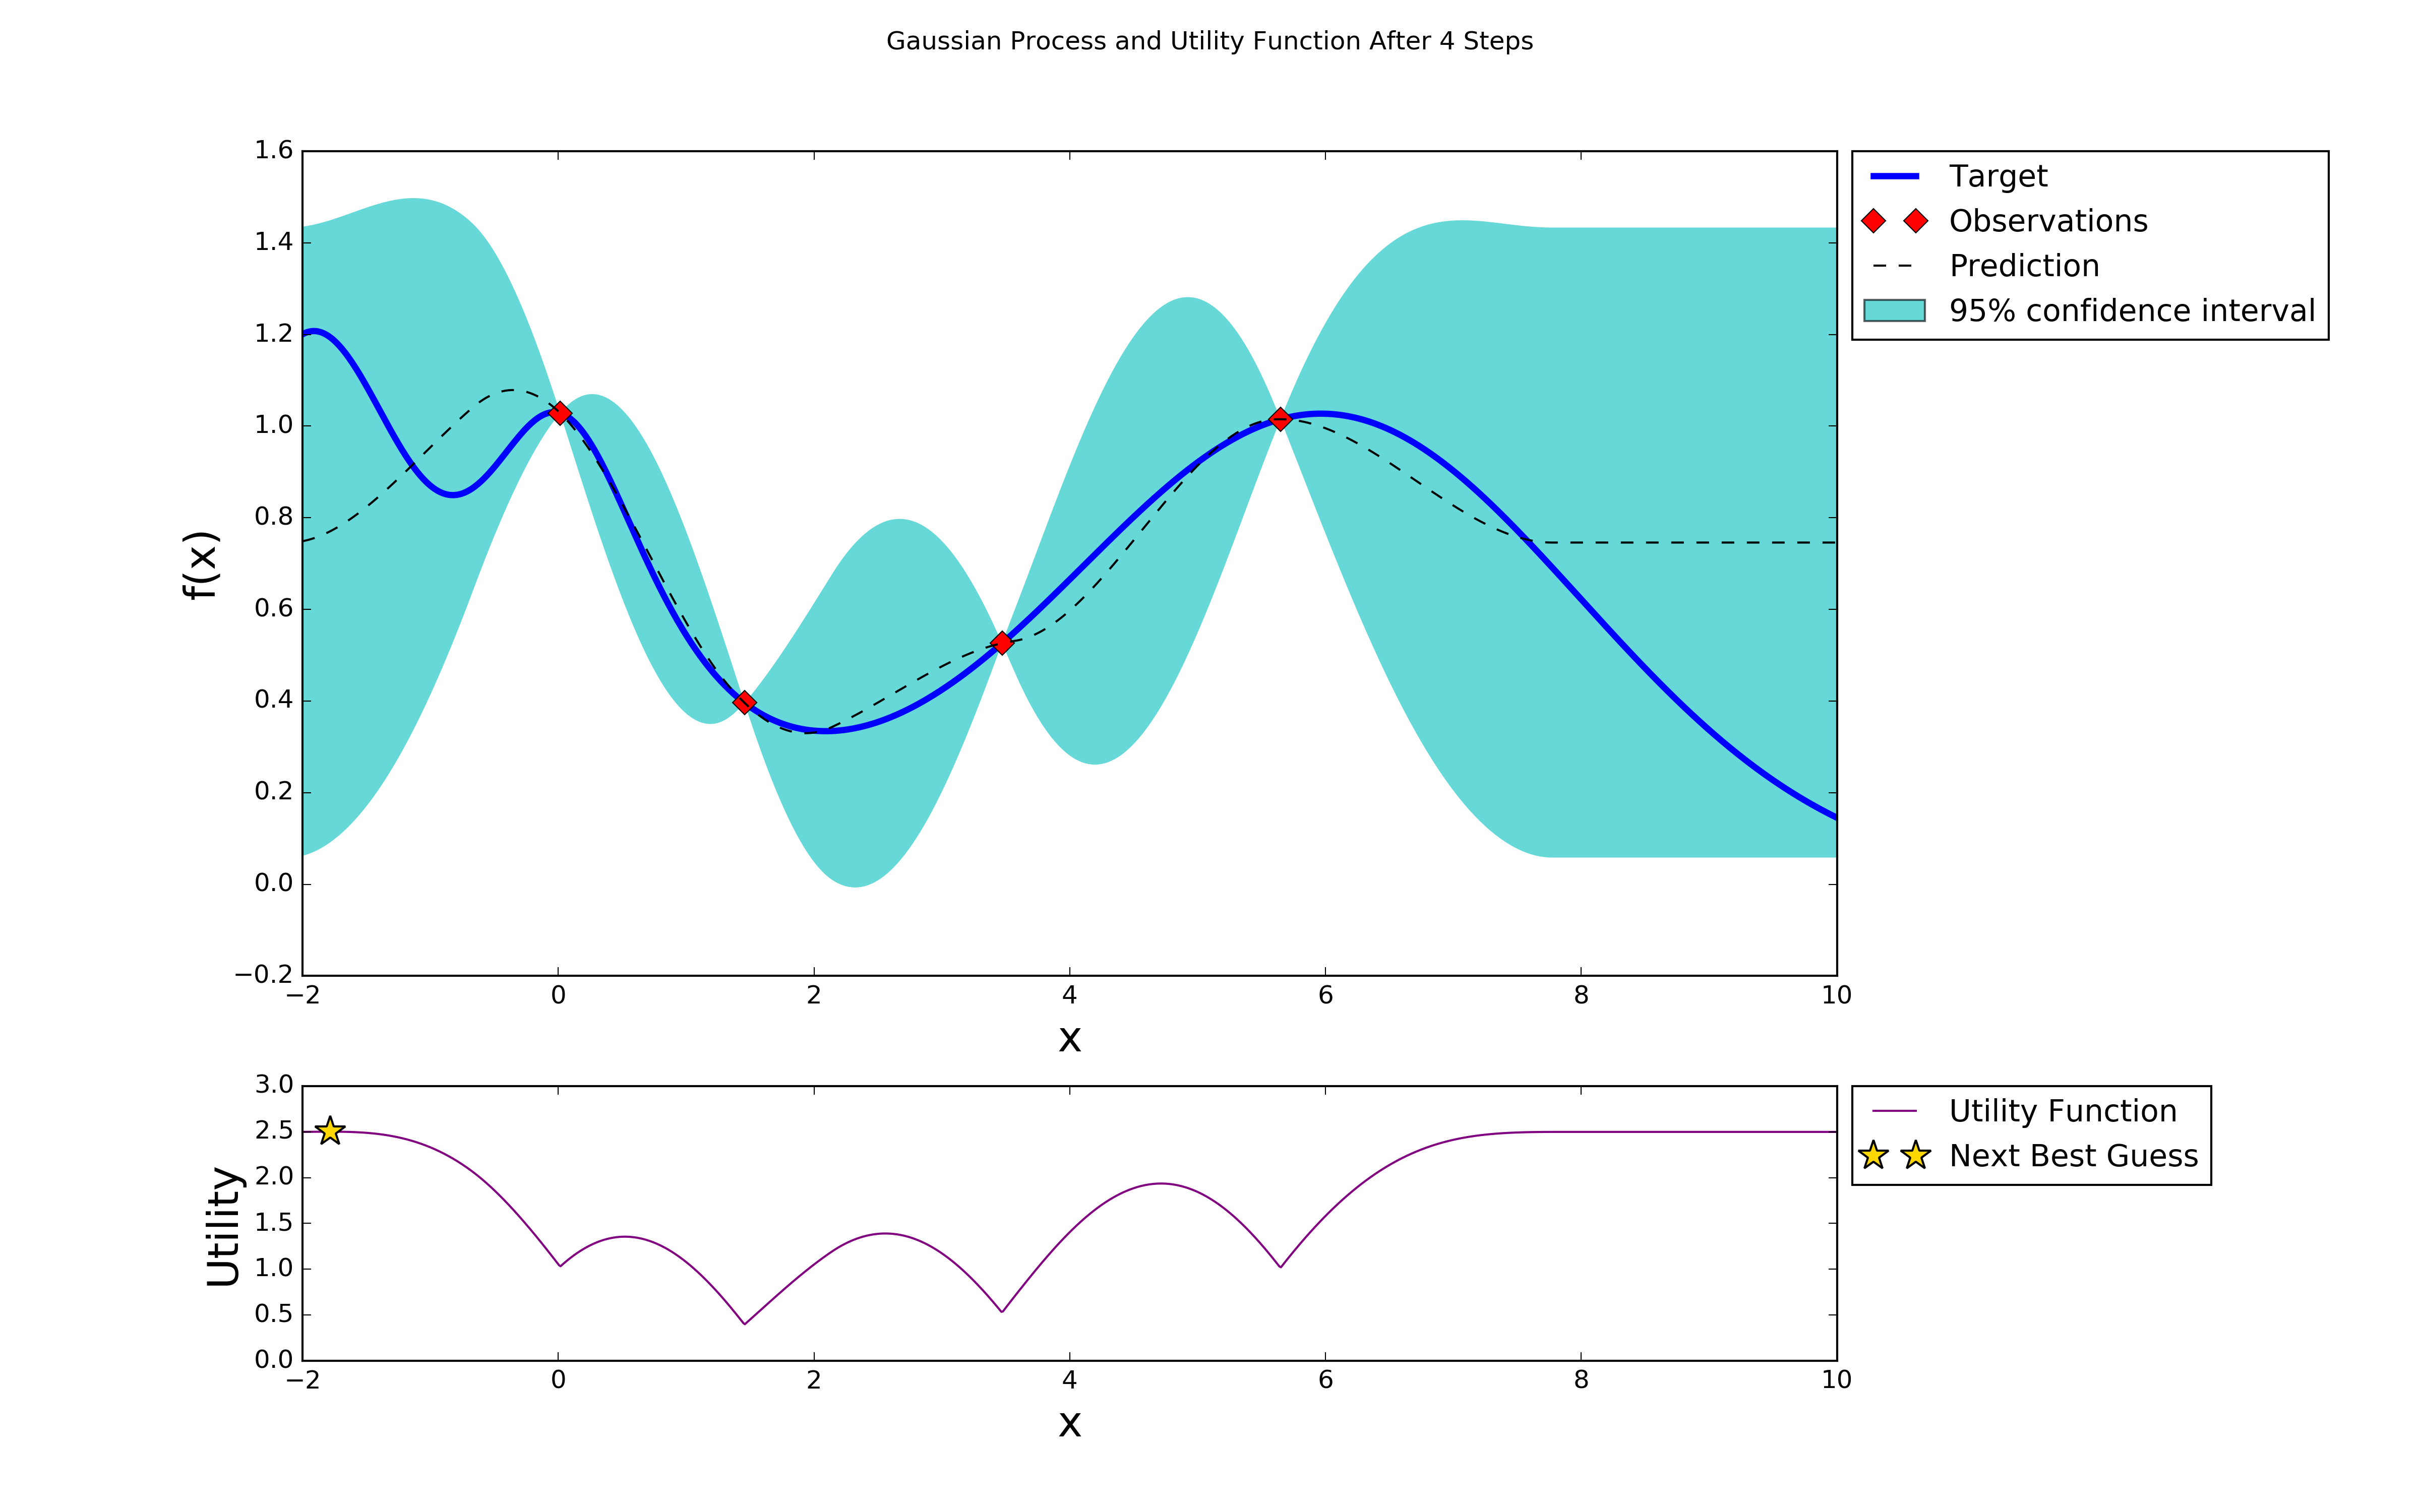
\includegraphics[width=1\textwidth]{figures/BO.png}
	\vspace{-2em}
	\caption{Example of an objective function and surrogate function. After probing observations from the objective functions the surrogate function is update to form the posterior. Uncertainty is low near observations.}
	\label{fig:bayesian-optimization}
\end{figure*}

\subsection{Kernel function}\label{sec:kernel-function}
The kernel is a function for the GP, which determines the smoothness of samples drawn from it. The choice of kernel is important in the process of fitting the Gaussian Process, to fit the objective function. Many kernels have been proposed, where one of the most used is the squared exponential function \citet{brochu2010tutorial}. The function however tends to smooth the surrogate function to much, to be applicable in real world problems. The kernel function used in this method will therefor be Matérn$\frac{5}{2}$, as proposed by \citet{snoek2012practical}.

\subsection{Acquisition function}\label{sec:acquisition-function}
When Bayesian optimization builds its model of the objective function, it iteratively choses inputs to sample outputs from the objective function. The choice of which inputs to sample from is determined by the \emph{acquisition function} (AF), which determines utility of sampling from a given input. Different acquisition functions yield different measures to make this decision. One measure is the \emph{Probability of Improvement} (PI) which given a candidate input computes the probability of improving the current best result. \todo{explain with figure} Another approach is to consider the \emph{expected improvement} (EI) which not only takes into account the probability of improvement, but also the uncertainty e.g. the variance of the Gaussian distribution of the surrogate at the given input.
EI balances the trade-off between exploitation and exploring, and is therefore a well used acquisiion function \citet{brochu2010tutorial}. $EI(x)$ is the function whch givs the expected improvement of choosing parameters x$x$, and is defines as:
\begin{equation}
\label{eq:expected-improvement}
EI(x) =
\begin{cases}
   (K + L & \text{ if } \sigma(x) > 0\\
   0 	  & \text{ if } \sigma(x) = 0
\end{cases}
\end{equation}
where $K = (\mu(x) - f(x^+))\Phi(Z)$ \\and $L = \sigma(x)\phi(Z)$ .
$\mu$ and $\sigma$ are the mean and variance of the posterior distribution of the surrogate function respectively, and $f(x^+)$ is the currently best result gained from probing the objective function. $Z$ is defined as:

\begin{equation}
\label{eq:expect-z}
Z =
\begin{cases}
\frac{\mu(x) - f(x^+)}{\sigma(x)} & \text{ if } \sigma(x) > 0\\
0 								  & \text{ if } \sigma(x) = 0
\end{cases}
\end{equation}
$\phi$ and $\Phi$ denote the \emph{probability density function} (PDF) and \emph{cumulative distribution function} (CDF) of the standard normal distribution.
The function for EI can then be used to probe the surrogate function with different parameter settings x, from where a new candidate point can be found to probe the objective function. The new candidate will be the parameter setting with the highest expected improvement.  

%- Combining posterior and refit the GP
